% Gemini theme
% https://github.com/anishathalye/gemini

\documentclass[
    final,
    ]{beamer}

% ====================
% Packages
% ====================

\usepackage[T1]{fontenc}
\usepackage{lmodern}
\usepackage[size=custom, width=120, height=67.5, scale=1.0]{beamerposter}
\usetheme{gemini}
\usecolortheme{gammapy}
\usepackage{graphicx}
\usepackage{booktabs}
\usepackage{tikz}
\usepackage{pgfplots}
\usepackage{fontawesome}
\setbeamerfont{caption name}{series=\bfseries}


\definecolor{monokaibg}{HTML}{272822}

% ====================
% Lengths
% ====================

% If you have N columns, choose \sepwidth and \colwidth such that
% (N+1)*\sepwidth + N*\colwidth = \paperwidth
\newlength{\sepwidth}
\newlength{\colwidth}
\setlength{\sepwidth}{0.025\paperwidth}
\setlength{\colwidth}{0.3\paperwidth}

\newcommand{\separatorcolumn}{\begin{column}{\sepwidth}\end{column}}
\newcommand{\coloredhref}[3][blue]{\href{#2}{\color{#1}{#3}}}%

% ====================
% Title
% ====================

\title{Gammapy: a Python Package for Gamma-Ray Astronomy}

\author{
    \textbf{Axel, Donath} \inst{1} \and
    \textbf{Regis, Terrier} \inst{2} \and
    Atreyee, Sinha \inst{3} \and
    Luca, Giunti \inst{4} \and
    Quentin, Remy \inst{1} \and
    Jose Enrique, Ruiz \inst{5} \and
    Fabio, Acero \inst{6} \and
    Fabio, Pintore \inst{7} \and
    Cosimo, Nigro \inst{8} \and
    Bruno, Khelifi  \inst{2} \and
    Laura Oliviera-Nieto  \inst{1} \and
    Maximilian, Noethe \inst{9} \and
    for the Gammapy developers
  }

\institute[shortinst]{
    \inst{1} MPIK, Heidelberg \samelineand
    \inst{2} APC, Paris \samelineand
    \inst{3} LUPM, Montpellier \samelineand
    \inst{4} CEA, Paris \samelineand
    \inst{5} IAA, Granada \samelineand
    \inst{6} CNRS, Paris \samelineand
    \inst{7} INAF-IASF, Palermo \samelineand
    \inst{8} IFAE, Barcelona \samelineand
    \inst{9} TU Dortmund, Dortmund
    }

% ====================
% Footer (optional)
% ====================

\footercontent{
  \href{https://www.gammapy.org}{https://www.gammapy.org.com} \hfill
  ICRC 2021, Berlin \hfill
  \href{mailto:alyssa.p.hacker@example.com}{alyssa.p.hacker@example.com}}
% (can be left out to remove footer)

% ====================
% Logo (optional)
% ====================

% use this to include logos on the left and/or right side of the header:
\logoright{
\includegraphics[height=7cm]{figures/logo/gammapy_logo_white.pdf}}
% \logoleft{\includegraphics[height=7cm]{logo2.pdf}}

% ====================
% Body
% ====================

\begin{document}

\begin{frame}[t]
\begin{columns}[t]
\separatorcolumn

\begin{column}{\colwidth}

  \begin{block}{Introduction \& Motivation}

    Some block contents, followed by a diagram, followed by a dummy paragraph.

    \begin{figure}
      \centering
      \begin{tikzpicture}[scale=6]
        \draw[step=0.25cm,color=gray] (-1,-1) grid (1,1);
        \draw (1,0) -- (0.2,0.2) -- (0,1) -- (-0.2,0.2) -- (-1,0)
          -- (-0.2,-0.2) -- (0,-1) -- (0.2,-0.2) -- cycle;
      \end{tikzpicture}
      \caption{A figure caption.}
    \end{figure}

    Lorem ipsum dolor sit amet, consectetur adipiscing elit. Morbi ultricies
    eget libero ac ullamcorper. Integer et euismod ante. Aenean vestibulum
    lobortis augue, ut lobortis turpis rhoncus sed. Proin feugiat nibh a
    lacinia dignissim. Proin scelerisque, risus eget tempor fermentum, ex
    turpis condimentum urna, quis malesuada sapien arcu eu purus.

  \end{block}

  \begin{block}{A block containing a list}

    Nam vulputate nunc felis, non condimentum lacus porta ultrices. Nullam sed
    sagittis metus. Etiam consectetur gravida urna quis suscipit.

    \begin{itemize}
      \item \textbf{Mauris tempor} risus nulla, sed ornare
      \item \textbf{Libero tincidunt} a duis congue vitae
      \item \textbf{Dui ac pretium} morbi justo neque, ullamcorper
    \end{itemize}

    Eget augue porta, bibendum venenatis tortor.

  \end{block}

  \begin{alertblock}{Install Gammapy}

    Thre recommanded way to install Gammapy is to \coloredhref[pink]{https://www.anaconda.com/products/individual}{download the Anaconda Python distribution} and then create a new virtual environment
    from the dedicated conda environment file:



  \end{alertblock}

\end{column}

\separatorcolumn

\begin{column}{\colwidth}

  \begin{block}{A block containing an enumerated list}

    Vivamus congue volutpat elit non semper. Praesent molestie nec erat ac
    interdum. In quis suscipit erat. \textbf{Phasellus mauris felis, molestie
    ac pharetra quis}, tempus nec ante. Donec finibus ante vel purus mollis
    fermentum. Sed felis mi, pharetra eget nibh a, feugiat eleifend dolor. Nam
    mollis condimentum purus quis sodales. Nullam eu felis eu nulla eleifend
    bibendum nec eu lorem. Vivamus felis velit, volutpat ut facilisis ac,
    commodo in metus.

    \begin{enumerate}
      \item \textbf{Morbi mauris purus}, egestas at vehicula et, convallis
        accumsan orci. Orci varius natoque penatibus et magnis dis parturient
        montes, nascetur ridiculus mus.
      \item \textbf{Cras vehicula blandit urna ut maximus}. Aliquam blandit nec
        massa ac sollicitudin. Curabitur cursus, metus nec imperdiet bibendum,
        velit lectus faucibus dolor, quis gravida metus mauris gravida turpis.
      \item \textbf{Vestibulum et massa diam}. Phasellus fermentum augue non
        nulla accumsan, non rhoncus lectus condimentum.
    \end{enumerate}

  \end{block}

  \begin{block}{Package Stucture}

    \begin{figure}
      \centering
      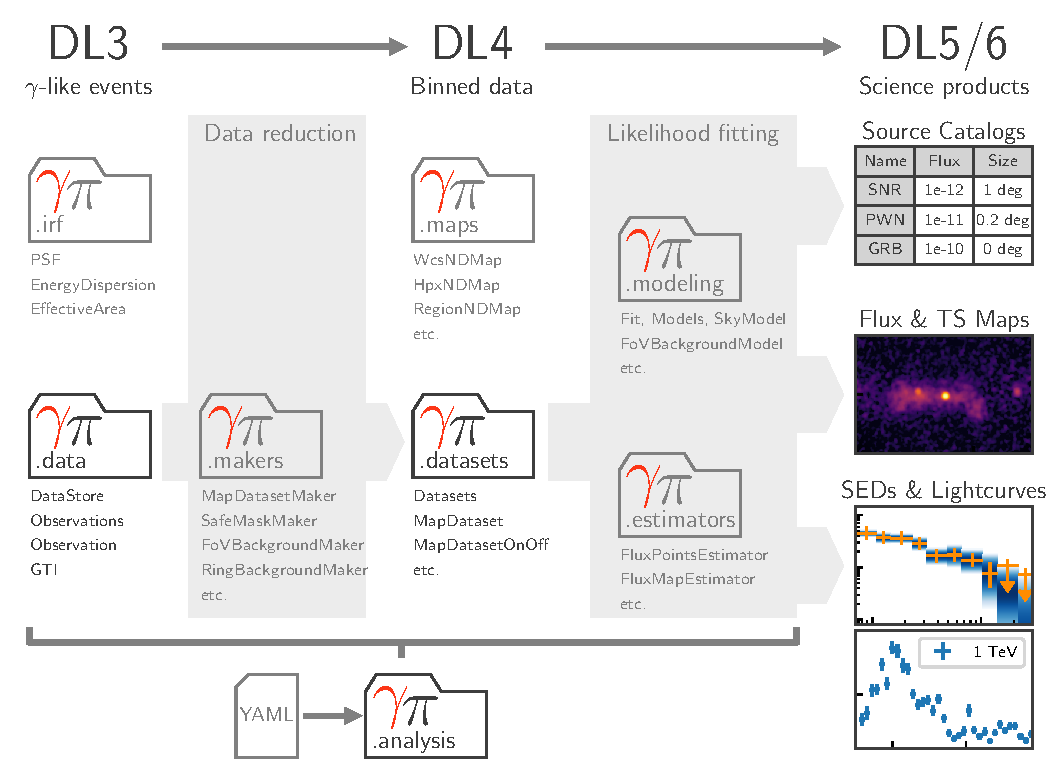
\includegraphics[width=\textwidth]{figures/data-flow-gammapy.pdf}
      \caption{Data flow and sub-package structure of Gammapy. The folder icons represent the corresponding sub-packages. The direction of the the data flow is illustrated with shaded arrows. The top section shows the data levels as defined by \coloredhref[pink]{https://www.cta-observatory.org}{CTA}.}
    \end{figure}

  Gammapy is structured into sub-packages.

  \end{block}

  % \begin{block}{Nam cursus consequat egestas}

  %   Nulla eget sem quam. Ut aliquam volutpat nisi vestibulum convallis. Nunc a
  %   lectus et eros facilisis hendrerit eu non urna. Interdum et malesuada fames
  %   ac ante \textit{ipsum primis} in faucibus. Etiam sit amet velit eget sem
  %   euismod tristique. Praesent enim erat, porta vel mattis sed, pharetra sed
  %   ipsum. Morbi commodo condimentum massa, \textit{tempus venenatis} massa
  %   hendrerit quis. Maecenas sed porta est. Praesent mollis interdum lectus,
  %   sit amet sollicitudin risus tincidunt non.

  %   Etiam sit amet tempus lorem, aliquet condimentum velit. Donec et nibh
  %   consequat, sagittis ex eget, dictum orci. Etiam quis semper ante. Ut eu
  %   mauris purus. Proin nec consectetur ligula. Mauris pretium molestie
  %   ullamcorper. Integer nisi neque, aliquet et odio non, sagittis porta justo.

  %   \begin{itemize}
  %     \item \textbf{Sed consequat} id ante vel efficitur. Praesent congue massa
  %       sed est scelerisque, elementum mollis augue iaculis.
  %       \begin{itemize}
  %         \item In sed est finibus, vulputate
  %           nunc gravida, pulvinar lorem. In maximus nunc dolor, sed auctor eros
  %           porttitor quis.
  %         \item Fusce ornare dignissim nisi. Nam sit amet risus vel lacus
  %           tempor tincidunt eu a arcu.
  %         \item Donec rhoncus vestibulum erat, quis aliquam leo
  %           gravida egestas.
  %       \end{itemize}
  %     \item \textbf{Sed luctus, elit sit amet} dictum maximus, diam dolor
  %       faucibus purus, sed lobortis justo erat id turpis.
  %     \item \textbf{Pellentesque facilisis dolor in leo} bibendum congue.
  %       Maecenas congue finibus justo, vitae eleifend urna facilisis at.
  %   \end{itemize}

  % \end{block}

\end{column}

\separatorcolumn

\begin{column}{\colwidth}

  \begin{block}{A block containing some math}

    Nullam non est elit. In eu ornare justo. Maecenas porttitor sodales lacus,
    ut cursus augue sodales ac.

    $$
    \int_{-\infty}^{\infty} e^{-x^2}\,dx = \sqrt{\pi}
    $$

    Interdum et malesuada fames $\{1, 4, 9, \ldots\}$ ac ante ipsum primis in
    faucibus. Cras eleifend dolor eu nulla suscipit suscipit. Sed lobortis non
    felis id vulputate.

    \heading{A heading inside a block}

    Praesent consectetur mi $x^2 + y^2$ metus, nec vestibulum justo viverra
    nec. Proin eget nulla pretium, egestas magna aliquam, mollis neque. Vivamus
    dictum $\mathbf{u}^\intercal\mathbf{v}$ sagittis odio, vel porta erat
    congue sed. Maecenas ut dolor quis arcu auctor porttitor.

    \heading{Another heading inside a block}

    Sed augue erat, scelerisque a purus ultricies, placerat porttitor neque.
    Donec $P(y \mid x)$ fermentum consectetur $\nabla_x P(y \mid x)$ sapien
    sagittis egestas. Duis eget leo euismod nunc viverra imperdiet nec id
    justo.

  \end{block}

  \begin{block}{Nullam vel erat at velit convallis laoreet}

    Class aptent taciti sociosqu ad litora torquent per conubia nostra, per
    inceptos himenaeos. Phasellus libero enim, gravida sed erat sit amet,
    scelerisque congue diam. Fusce dapibus dui ut augue pulvinar iaculis.

    \begin{table}
      \centering
      \begin{tabular}{l r r c}
        \toprule
        \textbf{First column} & \textbf{Second column} & \textbf{Third column} & \textbf{Fourth} \\
        \midrule
        Foo & 13.37 & 384,394 & $\alpha$ \\
        Bar & 2.17 & 1,392 & $\beta$ \\
        Baz & 3.14 & 83,742 & $\delta$ \\
        Qux & 7.59 & 974 & $\gamma$ \\
        \bottomrule
      \end{tabular}
      \caption{A table caption.}
    \end{table}

    Donec quis posuere ligula. Nunc feugiat elit a mi malesuada consequat. Sed
    imperdiet augue ac nibh aliquet tristique. Aenean eu tortor vulputate,
    eleifend lorem in, dictum urna. Proin auctor ante in augue tincidunt
    tempor. Proin pellentesque vulputate odio, ac gravida nulla posuere
    efficitur. Aenean at velit vel dolor blandit molestie. Mauris laoreet
    commodo quam, non luctus nibh ullamcorper in. Class aptent taciti sociosqu
    ad litora torquent per conubia nostra, per inceptos himenaeos.

    Nulla varius finibus volutpat. Mauris molestie lorem tincidunt, iaculis
    libero at, gravida ante. Phasellus at felis eu neque suscipit suscipit.
    Integer ullamcorper, dui nec pretium ornare, urna dolor consequat libero,
    in feugiat elit lorem euismod lacus. Pellentesque sit amet dolor mollis,
    auctor urna non, tempus sem.

  \end{block}

  \begin{block}{References}

    \nocite{*}
    \footnotesize{\bibliographystyle{plain}\bibliography{poster}}

  \end{block}

\end{column}

\separatorcolumn
\end{columns}
\end{frame}

\end{document}
